% assignment_2.tex - Assignment 2 for Machine Learning class (Spring 2015)
% Chanmann Lim - February 2015

\documentclass[a4paper]{article}

\usepackage[margin=1 in]{geometry}
\usepackage{amsmath}
\usepackage{listings}
\usepackage{graphicx}
\usepackage[T1]{fontenc}
\usepackage{float}

\everymath{\displaystyle}

\begin{document}

\subsection*{4. }

% ------------------------------------------ Part I ------------------------------------------
\paragraph{Part I:}
\paragraph{d.} Plot the data samples in \textbf{2DGaussianDataset1.txt} and decision boundary: \\
\begin{figure}[H]
  \centering
    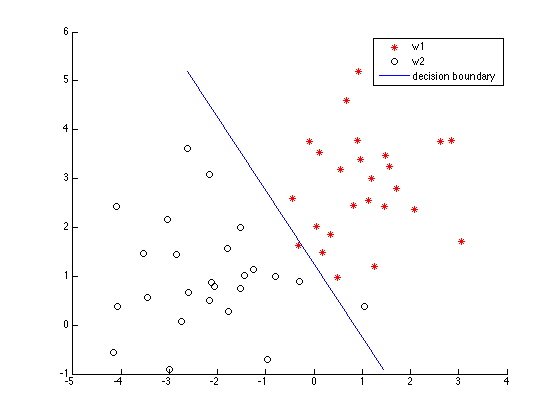
\includegraphics[scale=.6]{images/1_d.png}
  \caption{\textbf{2DGaussianDataset1.txt} and decision boundary (Classifier 1)}
\end{figure}

\paragraph{e.} Plot $g(\underline{X}_{n})$ values: \\
\begin{figure}[H]
  \centering
    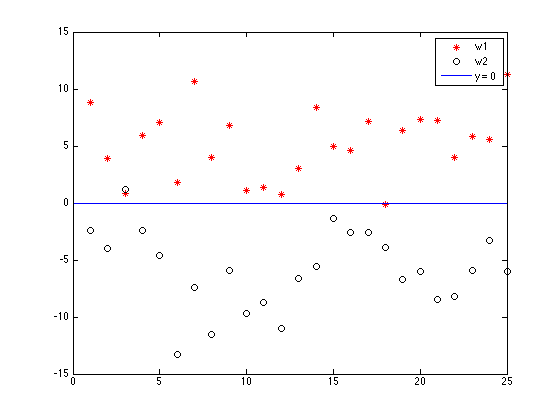
\includegraphics[scale=.6]{images/1_e.png}
  \caption{\textbf{2DGaussianDataset1.txt} and $g(\underline{X}_{n})$ values (Classifier 1)}
\end{figure}

\paragraph{e.} The classification error rate for classifier 1 with \textbf{2DGaussianDataset1.txt} = 4\%.

% ------------------------------------------ Part II ------------------------------------------
\paragraph{Part II:}
\paragraph{d.} Plot the data samples in \textbf{2DGaussianDataset2.txt} and decision boundary: \\
\begin{figure}[H]
  \centering
    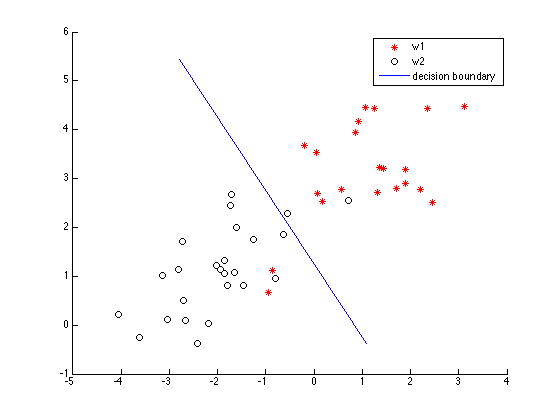
\includegraphics[scale=.6]{images/2_d.png}
  \caption{\textbf{2DGaussianDataset2.txt} and decision boundary (Classifier 1)}
\end{figure}

\paragraph{e.} Plot $g(\underline{X}_{n})$ values: \\
\begin{figure}[H]
  \centering
    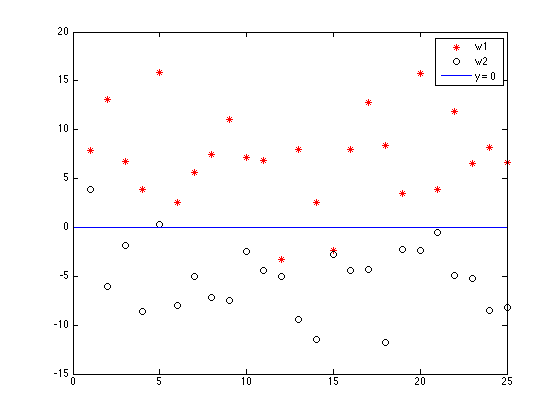
\includegraphics[scale=.6]{images/2_e.png}
  \caption{\textbf{2DGaussianDataset2.txt} and $g(\underline{X}_{n})$ values (Classifier 1)}
\end{figure}

\paragraph{e.} The classification error rate for classifier 1 with \textbf{2DGaussianDataset2.txt} = 8\%.

% ------------------------------------------ Part III ------------------------------------------
\paragraph{Part III:}
\paragraph{d.} Plot the data samples in \textbf{2DGaussianDataset2.txt} and decision boundary: \\
\begin{figure}[H]
  \centering
    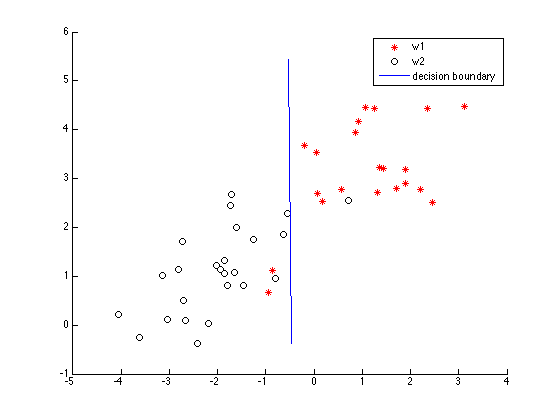
\includegraphics[scale=.6]{images/3_d.png}
  \caption{\textbf{2DGaussianDataset2.txt} and decision boundary (Classifier 2)}
\end{figure}

\paragraph{e.} Plot $g(\underline{X}_{n})$ values: \\
\begin{figure}[H]
  \centering
    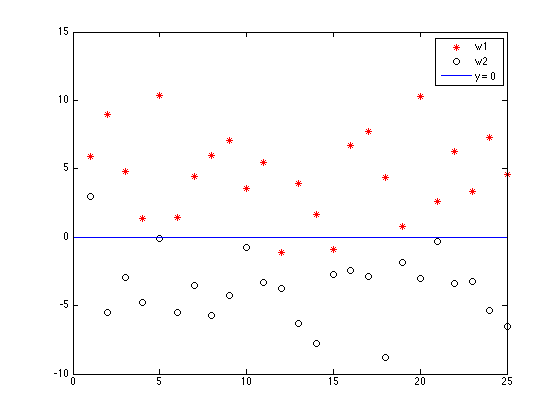
\includegraphics[scale=.6]{images/3_e.png}
  \caption{\textbf{2DGaussianDataset2.txt} and $g(\underline{X}_{n})$ values (Classifier 2)}
\end{figure}

\paragraph{e.} The classification error rate for classifier 2 with \textbf{2DGaussianDataset2.txt} = 6\%. \\

% ------------------------------------------ Explain ------------------------------------------
The difference between the error rates in \textbf{Part II} and \textbf{Part III} on \textbf{2DGaussianDataset2.txt} is due to the classifiers being used to perform the classification task. Classifier 2 is more accurate than classifier 1 since there is additional information available in term of correlation in the given covariance matrix in classifier 2. \\

\begin{align*}
\Sigma_{classifier\_1} = 
	\begin{bmatrix}
		1.21 & 0 \\
		0 & 1.21
	\end{bmatrix} \\ \\
\Sigma_{classifier\_2} = 
	\begin{bmatrix}
		1.21 & 0.8 \\
		0.8 & 1.21
	\end{bmatrix}
\end{align*}

\newpage
\subsection*{Appendix:}
\lstinputlisting[language=Matlab, title=\lstname, basicstyle=\footnotesize]{assignment_2.m}
\lstinputlisting[language=Matlab, title=\lstname, basicstyle=\footnotesize]{report.m}
\lstinputlisting[language=Matlab, title=\lstname, basicstyle=\footnotesize]{MAP.m}
\lstinputlisting[language=Matlab, title=\lstname, basicstyle=\footnotesize]{classify.m}
\lstinputlisting[language=Matlab, title=\lstname, basicstyle=\footnotesize]{decision_boundary.m}

\end{document}